% !TEX root = ../sbgn_ER-level1.tex
% =============================================================================
% overview
% =============================================================================

\section{Overview of the Entity Relationship language}\label{sec:overview}

To set the stage for what follows in this chapter, we first give a brief overview of some of the concepts in the \ER language with the help of an example shown in \fig{eg1}. 

\begin{figure}[H]
  \centering
  \vspace*{-0.75em}
  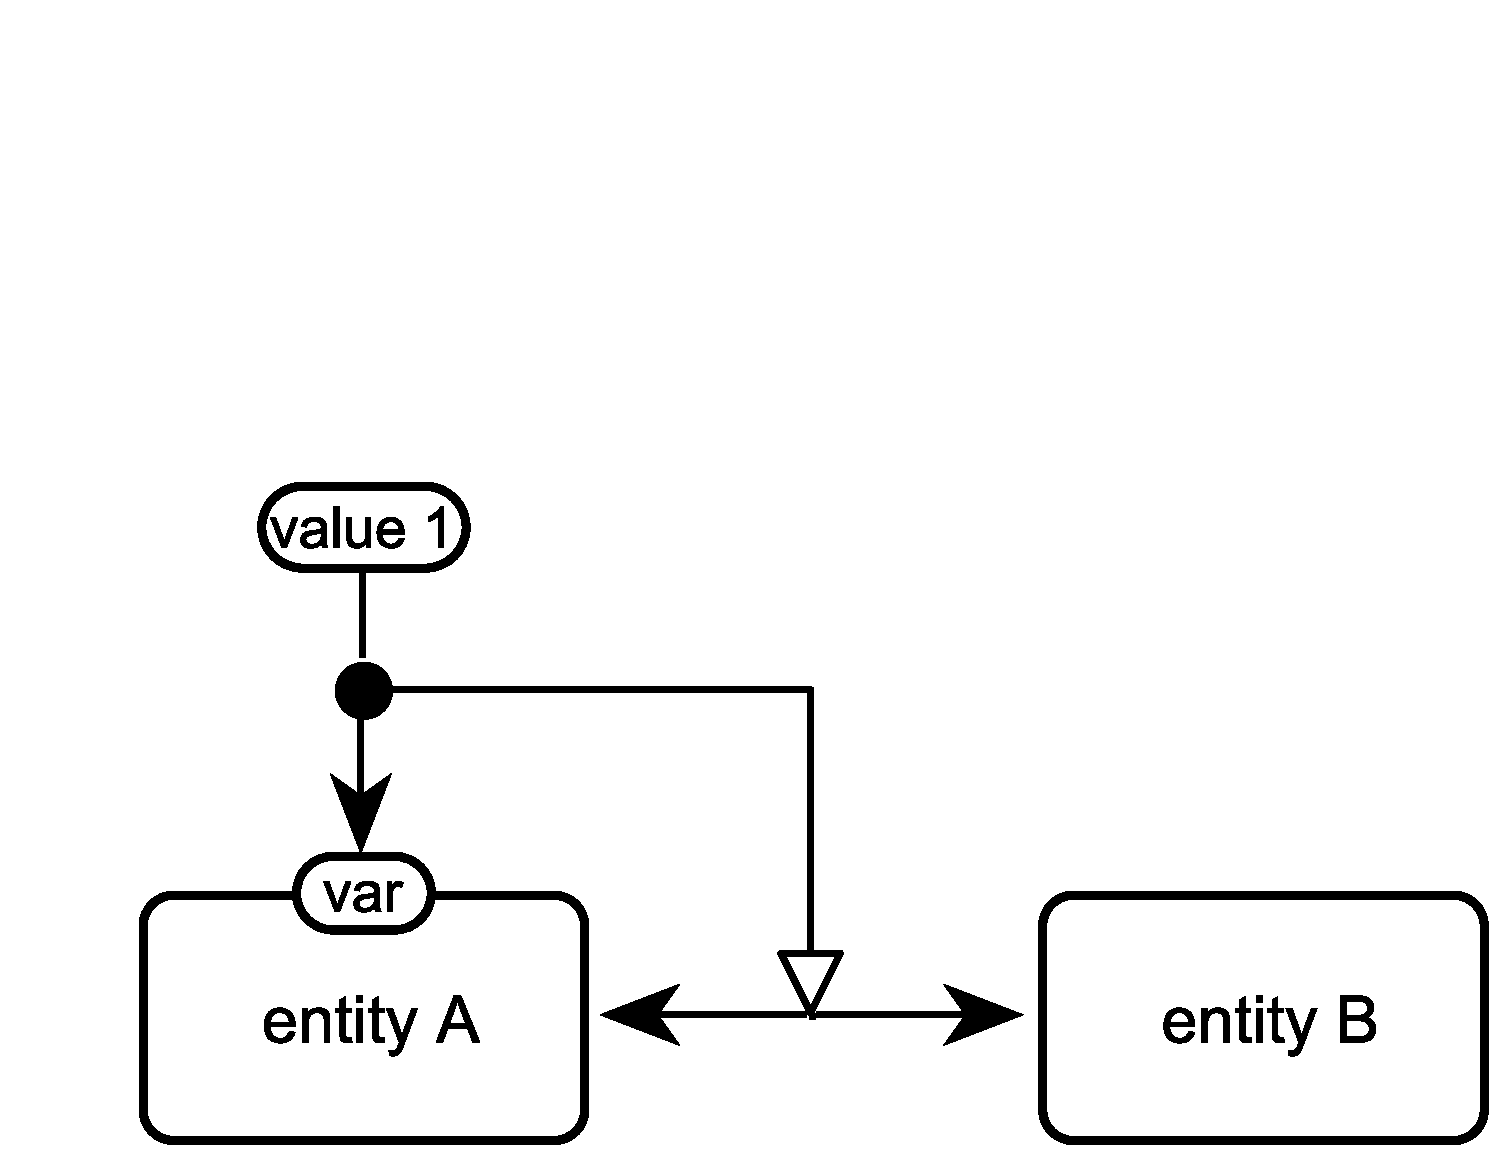
\includegraphics[scale=0.45]{examples/HelloWorld}
   \caption{This example of an \ERm represents an entity A interacting with another entity B. The assignment of value 1 to the state variable var of the entity A stimulates the interaction between entity A and entity B.}
  \label{fig:eg1}
\end{figure}

The essence of the \ERs is to depict the influences of entities upon the behaviour of others. The entities are classes of things that can exist, either on their own, or when statements (interactions and assignments) become true, so existence is the key concept in \ERs. For entity to participate in relationship at least one of it's instance should exist. Instances of different entities can interact (such as ``entity A'' and ``entity B'' in \fig{eg1}), or a value can be assigned to a property of some instance of an entity (such as ``value 1'' to property ``var'' of ``entity A'' in \fig{eg1}). The entities can modify the interactions between other entities, for example, stimulation of the interaction between ``entity A'' and ``entity B'' in \fig{eg1} takes place if ``value 1'' is really assigned to property ``var'' of some instance of the ``entity A''. The existence of the assignment (set of instances where value is really assigned to the property) is represented by the black dot (called \glyph{outcome}). The influences can therefore be understood as logical consequences of existence of participating instances.  On the contrary to the \PDl, where the different processes affect each other in a way that the behaviour of the depicted system can only be understood taking into account the whole system, the relationships are essentially independent. One can imagine that each of the relationships represents a specific conclusion of a scientific experiment reported in an article. Their addition on a map represents the knowledge we have of the effects of the entities represented upon each other. In  \fig{eg1}, we have three statements: 

\begin{itemize}
 \item ``entity A'' can interact with ``entity B''.
 \item property ``var'' of ``entity A'' can take the value ``value 1''.
 \item if ``var'' is set to ``value 1'', the interaction between ``entity A'' and ``entity B'' is stimulated.
\end{itemize}


The independence of relationships in \ERs is the key to avoid the combinatorial explosions inherent to \PDs.

A more complex and realistic example of \ERm is shown in \fig{eg2}. This example will be re-used throughout the description of the graphical symbols (glyphs) used by \SBGNERLone (with a few additions when the concepts are missing in the example) 

\begin{figure}[H]
  \centering
  \vspace*{-0.75em}
  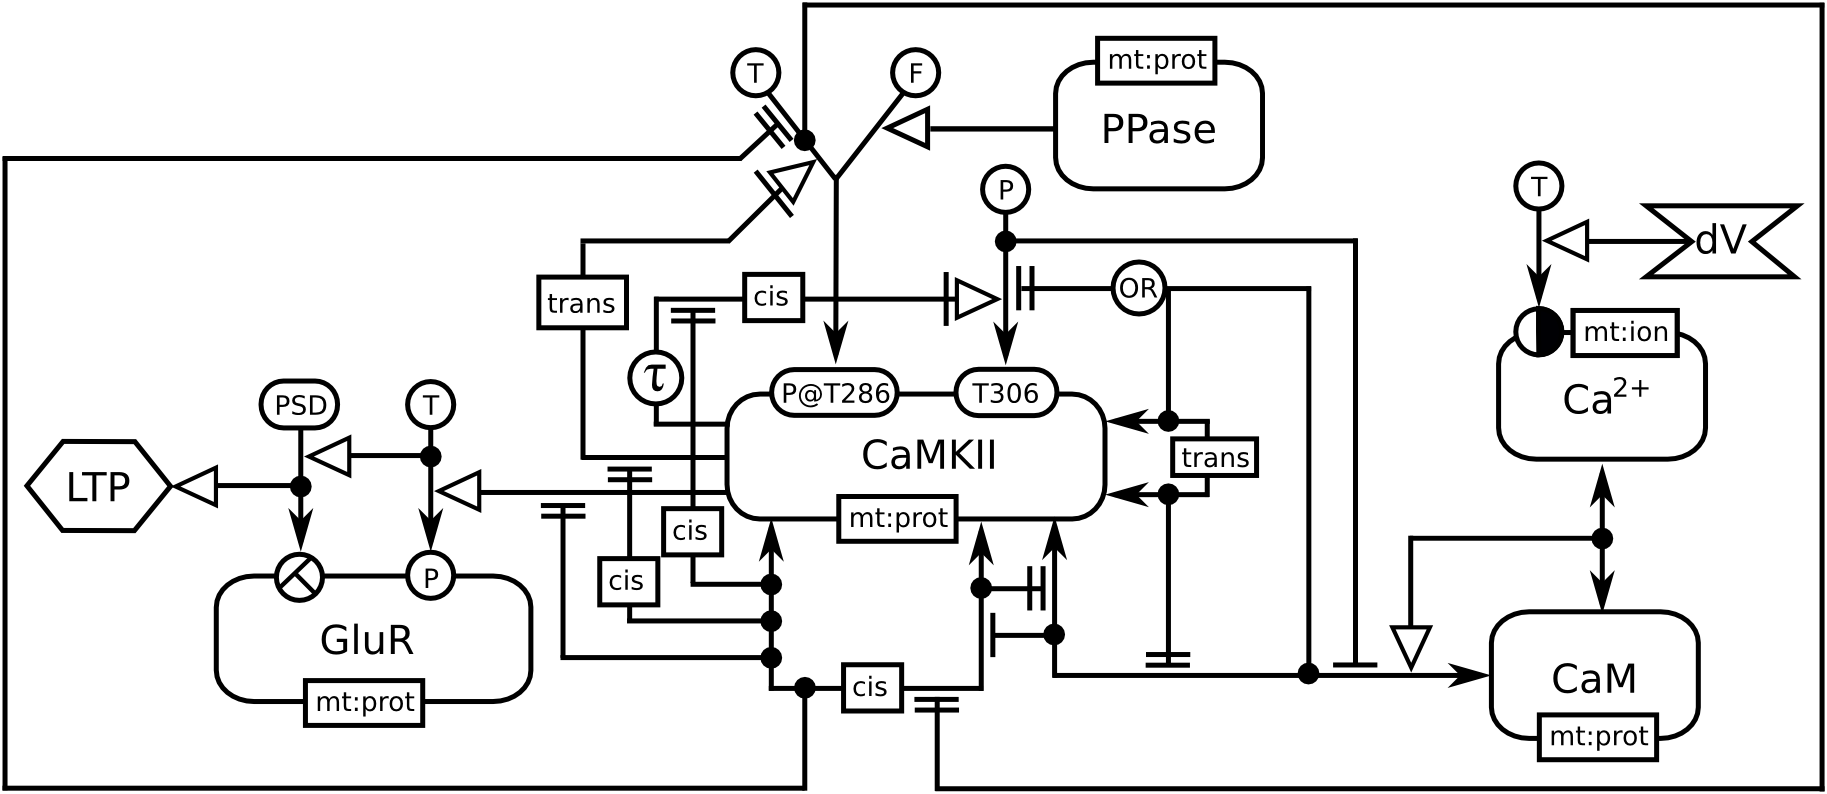
\includegraphics[scale=0.45]{examples/CaMKII-intro}
   \caption{This example of an \ERm depicts the effect of a depolarisation (dV) on the intracellular calcium, that binds to calmodulin, that itself binds to the calcium/calmoduline kinase II (CaMKII). The binding of calmodulin inhibits the folding of CaMKII monomer on itself, thus relieving the inhibition on the kinase activity. The phosphorylation of the glutamate receptors finally leads to the Long Term Potentiation (LTP) of the synapses. In addition, the map shows the effect of trans-phosphorylation on threonine 286, that makes the enzyme constitutively active, and on threonine 306, that renders the kinase insensitive to calmodulin, as well as the dimerisation of the kinase.}
  \label{fig:eg2}
\end{figure}
 


\tab{component-summary} summarizes the different SBGN abstractions described in this chapter.
 
\newcolumntype{P}[1]{>{\raggedright\hspace{0pt}\arraybackslash}p{#1}}
 
 \begin{table}[h]
   \centering
   \small
   \begin{tabular}{@{}lP{2.4in}P{2.4in}@{}}
     \toprule
     \textbf{Component} & \textbf{Role} & \textbf{Examples}\\
     \midrule
     Entity node
     & Something that exists, whether a physical object or sets of objects.  
     & An entity, the result of an interaction \\[0.5em]
 
     Statement arc
     & Something that can be true or false, and affects or relates entities.
     & An interaction between entities, the assignment of a value to a variable \\[0.5em]
 
     Influence
     & The effect of something true on the realisation of a statement or another influence.
     & A stimulation, an absolute inhibition \\
     \bottomrule
   \end{tabular}
   \caption{Summary of \ER components and their roles.}
   \label{tab:component-summary}
 \end{table}

